\chapter{Methodology for mapping NAPLAN scale scores to comparative year levels} \label{chap3}

\section{Introduction}

The NAPLAN scale is designed to be independent of year level -- a student should receive the same score on average regardless of whether they take a test normally administered to Year 3, Year 5, Year 7 or Year 9 students.\footnote{A student's NAPLAN scale score will generally be a more precise estimate of their true ability when they are administered an age-appropriate test. Giving a typical Year 3 student a test meant for Year 9 students is likely to produce a NAPLAN scale score with a large standard error.} This property makes it possible to compare students in different test-taking year levels. For example, a Year 5 student is predicted to be above Year 7 standard if they score higher than the typical Year 7 student. But because NAPLAN tests are only administered to students in four different year levels, it is not possible to compare students to those outside these year levels without further assumptions.

\textit{Closing the gaps} presents a new framework from which to interpret NAPLAN results. NAPLAN scale scores are mapped onto a new measure, \textit{comparative year levels}. The NAPLAN scale score corresponding to the comparative year level 4, for example, is the median score expected from students if they took an age-appropriate NAPLAN test when they were in Year 4.\footnote{To be precise, in May of the year they were in Year 4, as this is when the NAPLAN test is taken.}  

This appendix outlines the theoretical framework for mapping NAPLAN scale scores onto comparative year levels and the methodology and assumptions used to estimate this relationship.

\section{Theoretical framework for mapping} \label{sec:theoretical}

Let $X_{j}$ ($X_{j} \in \mathbb{R}$) be a random variable denoting student ability (as estimated by NAPLAN scale scores) in domain ${j}$ ($j = $ reading, numeracy), and $Y$ be a variable denoting schooling year level, continuous over the range of schooling years, $\left(y_{min},y_{max}\right)$.\footnote{Lower case letters are used to denote realisations of these random variables. This report's analysis focuses on reading and numeracy only, but it would be possible to apply the same analysis to the other assessment domains.}

We assume that median student ability increases monotonically as students progress through school. We define a function $f_{j}(Y)$ as the median of $X_{j}$ conditional on $Y$:
\newcommand\numberthis{\addtocounter{equation}{1}\tag{\theequation}}
\begin{align*}
 f_{j}(Y) &= Q_{50}\left[X_{j} \mid Y\right]  \\ 
 y_1 < y_2 &\implies f_{j}(y_{1}) < f_{j}(y_{2}) \numberthis\label{eq:median} \\ 
 f_{j}(Y) &\in f_{j}\left[y_{\min},y_{\max}\right] 
\end{align*}
%\begin{equation} \begin{array}{c} Q_{50}\left[X_{j} | Y\right] = f_{j}(Y) \\ f_{j}(y_{1}) < f_{j}(y_{2}) \ \forall \ y_{1} < y_{2} \\ f_{j}(Y) \in \left(f_{j}[y_{min}],f_{j}[y_{max}]\right) \label{eq:median}
%\end{array} \end{equation}
That is, $f_{j}(Y)$ is the median NAPLAN scale score in domain ${j}$ of students taking a NAPLAN test in year level $Y$. For every schooling level there is a corresponding median NAPLAN scale score (for each domain). We also assume that $f_{j}(Y)$ is continuous and monotonically increasing -- at the population level, median student ability increases steadily over time.\footnote{For example, if NAPLAN tests were taken every month, we would expect the median score to improve with every test. This may not hold for individual students, but should hold at the population level.}

Following this, we propose that a given NAPLAN scale score corresponds to a median schooling year -- the point in time in the median student's path of progress (in terms of year level and months) at which their ability is equal to that score. We define this schooling year as a \textit{comparative year level}, denoted as $Y^{*}$:
\begin{equation} Y^{*} = f_{j}^{-1}\left(X_{j}\right) 
\end{equation}
All NAPLAN scale scores in the range $\left(f_{j}[y_{min}],f_{j}[y_{max}]\right)$ therefore correspond to a \textit{comparative year level}.

\section{Estimating comparative year levels}

This methodology aims to estimate $f_{j}(Y)$ for reading and numeracy at each schooling year level, $Y = 1,2,...,12$, then interpolate over these points to construct a smooth curve. If the NAPLAN tests were administered to students in every year level (from Year 1 to Year 12), this would be straightforward -- $\widehat{f}_{j}(Y)$ would just be the sample median from each year level. But with the tests only administered in four year levels, we must make further assumptions to estimate $f_{j}(Y)$.

The report estimates $f_{j}(Y)$ (the median NAPLAN scale scores corresponding to a given year level) using the simulated NAPLAN results (see Section \ref{sec:pv}) of all Australian students in 2014 linked to their 2012 simulated results (where applicable). It is possible to apply this methodology to NAPLAN results in other years, provided linked data are available.

\textbf{Step 1: Estimate the corresponding NAPLAN scale scores for comparative year levels 3, 5, 7, and 9}
\nopagebreak

These are estimated as the sample median scores in those year levels:
\begin{equation} \begin{array}{c}
\widehat{f}_{j}(3) = \tilde{x}_{j,3} \vspace{0.3em}\\ \widehat{f}_{j}(5) = \tilde{x}_{j,5} \vspace{0.3em}\\ \widehat{f}_{j}(7) = \tilde{x}_{j,7} \vspace{0.3em}\\ \widehat{f}_{j}(9) = \tilde{x}_{j,9}
\end{array} \end{equation}
where $\tilde{x}_{j,y}$ is the sample median NAPLAN scale score in year level $y$.\footnote{For Years 3, 5, and 7, we estimated the corresponding NAPLAN scale score, $\widehat{f}_{j}(Y)$, as the average of the medians in 2012 and 2014.}

\textbf{Step 2: Interpolate between Year 3 and Year 9}
\nopagebreak

Using a third-order polynomial, fit a smooth curve through the four data points, ($[Y,\widehat{f}_{j}(Y)], Y = 3,5,7,9$), to estimate $f_{j}(Y)$ between Year 3 and Year 9, as shown in \Cref{fig:interpolation}.

\begin{figure}[t]
 \captionwithunits{A third-order polynomial is used to interpolate between Year 3 and Year 9}{Estimated median NAPLAN scale score, $\widehat{f}_{j}(Y)$, numeracy}
 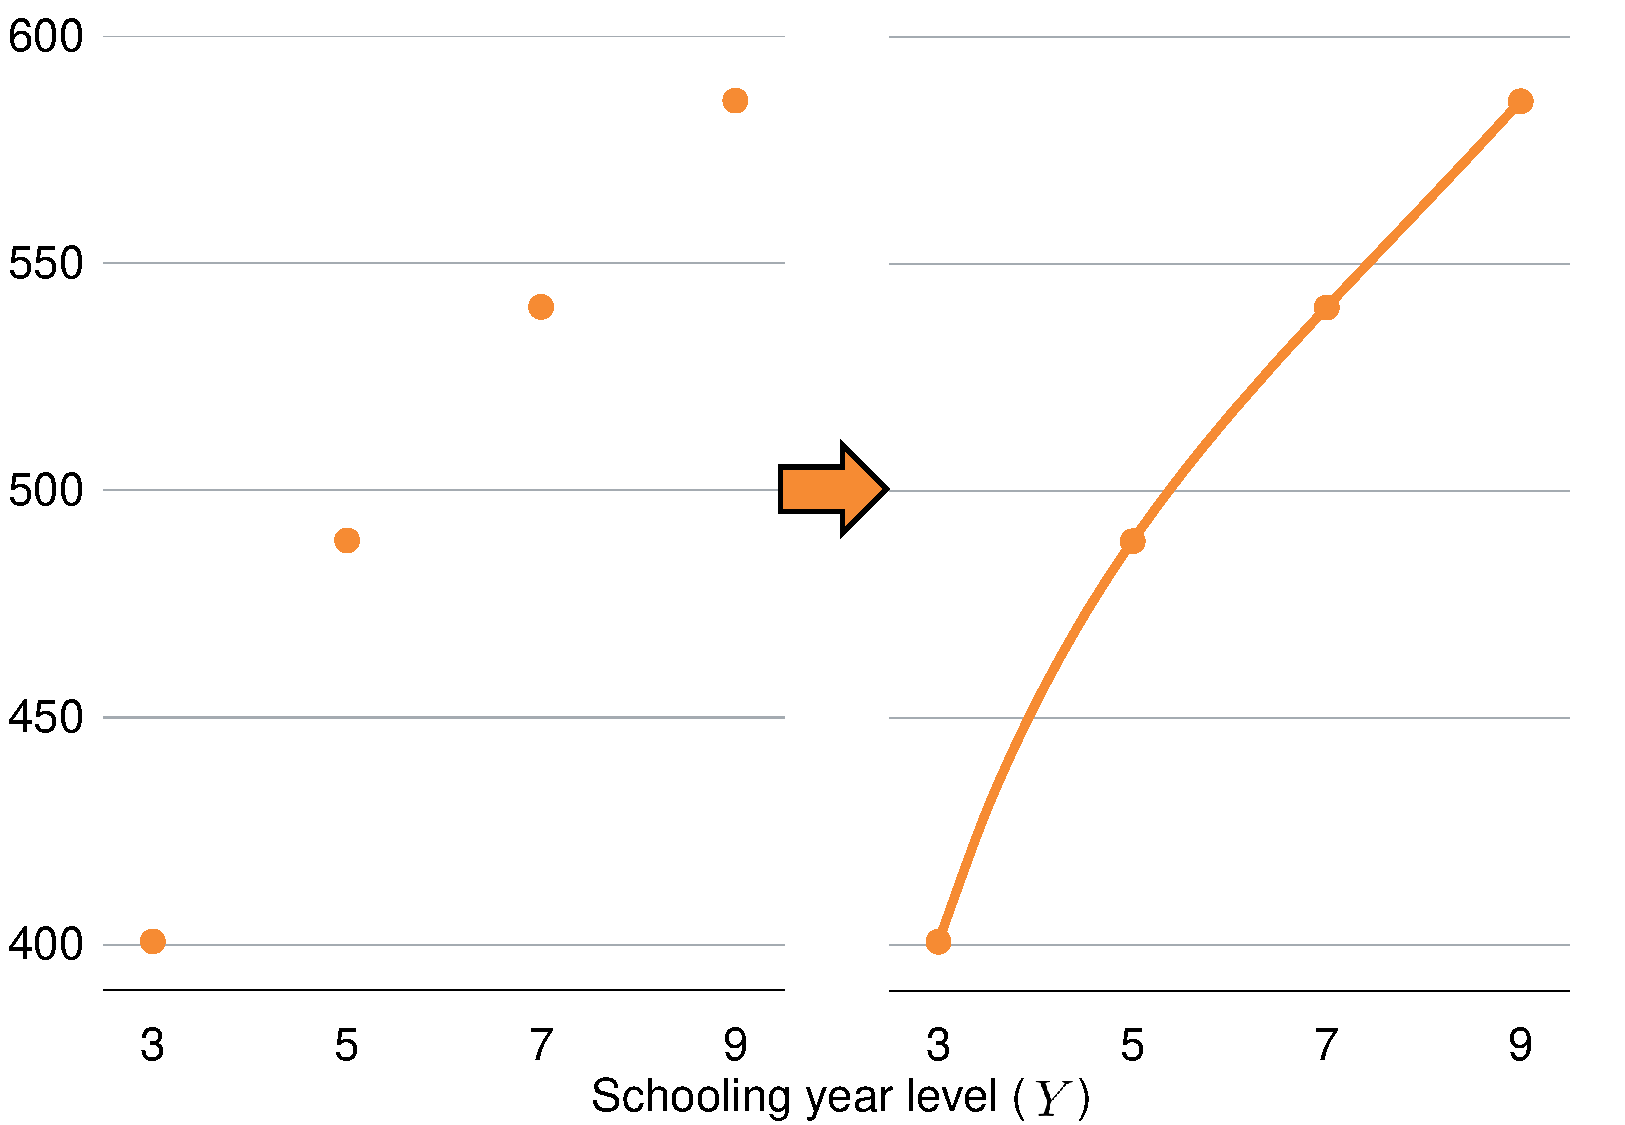
\includegraphics[width=\columnwidth]{atlas/Interpolation.pdf}\label{fig:interpolation}

\source{Grattan analysis of \textcite{acara2014}.}
\end{figure}

This interpolation could be extrapolated to year levels below 3 and above 9, but this is unlikely to provide the best estimate of $f_{j}(Y)$ at such points. Instead, our approach takes into account the gain in NAPLAN scores as students progress through school.

We denote a function, $g_{j,Y}\left(X_{j,Y-2} \right)$, equal to the median gain score conditional on year level and NAPLAN scale score from two years earlier:
\begin{equation}
g_{j,Y}\left(X_{j,Y-2} \right) = Q_{50}\left[X_{j,Y}-X_{j,Y-2} | Y, X_{j,Y-2} \right] \label{eq:med_gain}
\end{equation}
where $X_{j,Y}$ denotes NAPLAN scale score in domain $j$ in school year $Y$. For students that scored $x_{j,3}$ in Year 3 reading, for example, $g_{j,5}(x_{j,3})$ is the median gain score these students will make to Year 5.\footnote{The function $g_{j,Y}$ can only be empirically estimated for $Y=5$, $7$ and $9$, corresponding to gain scores from Years 3 to 5, Years 5 to 7, and Years 7 to 9 respectively.}   

From \cref{eq:med_gain,eq:median}, it follows that:
\begin{equation} 
g_{j,Y}\left[f_{j}(Y-2)\right] = f_{j}(Y) - f_{j}(Y-2) \label{eq:gf}
\end{equation}
That is, the difference between the median scores two years apart is equal to the median gain made from the same starting score.

\textbf{Step 3: Estimate the median gain score curves for Years 3 to 5 and Years 7 to 9} 
\nopagebreak

To estimate $g_{j,Y}$ for $Y=5$ and $Y=9$ first requires parameterising the functions. We allow for non-linearity in $g_{j,Y}$ by using restricted cubic regression splines, meaning that $g_{j,Y}$ can be written as a linear function:
\begin{equation} \begin{array}{c}
g_{j,Y}(X_{j,Y-2}) = \beta_{0} + \beta_{1}X_{j,Y-2} + \beta_{2}S_{2}(X_{j,Y-2}) \vspace{0.3em}\\
+ \beta_{3}S_{3}(X_{j,Y-2}) + \beta_{4}S_{4}(X_{j,Y-2}) \label{eq:g_jY}
\end{array} \end{equation}
where $S_{2},S_{3}$ and $S_{4}$ are functions that create spline variables.\footnote{More spline variables can be included, if desired.} Alternatively, this function could be specified with quadratic or higher order polynomial terms.

Given $g_{j,Y}$ represents a conditional median gain score, \cref{eq:g_jY} can be thought of as a quantile regression model at the median. This can be estimated using least absolute deviations.\footnote{It is only necessary to estimate $g_{j,5}$ for $x_{j,3}\leq \widehat{f}_{j}(3)$ and $g_{j,9}$ for $x_{j,7} \geq \widehat{f}_{j}(7)$.}

\Cref{fig:g579} plots the estimated functions, $\widehat{g}_{j,y}\left(x_{j,y-2}\right)$, for $y=5,7$ and $9$ for both reading and numeracy. Predicted median NAPLAN gain scores are much higher for lower prior scores, but year level appears to have little effect on gain scores once prior scores are controlled for. For instance, when evaluated at the NAPLAN score for comparative year level 3, $\widehat{f}_{j}\left(3\right)$, the functions $\widehat{g}_{j,5}$ and $\widehat{g}_{j,7}$ are very close. Similarly, when evaluated at comparative year level 7, $\widehat{f}_{j}\left(7\right)$, the functions $\widehat{g}_{j,9}$ and $\widehat{g}_{j,7}$ are very close.\footnote{These functions are also very close when evaluated at comparative year level 9.} That is, expected NAPLAN gain from a given starting point is similar for students that are two year levels apart.

\begin{figure}[t]
 \captionwithunits{The estimated median gain score is strongly related to prior score, but only weakly related to year level}{Two-year median NAPLAN gain score, $\widehat{g}_{j,y}(x_{j,y-2})$}
 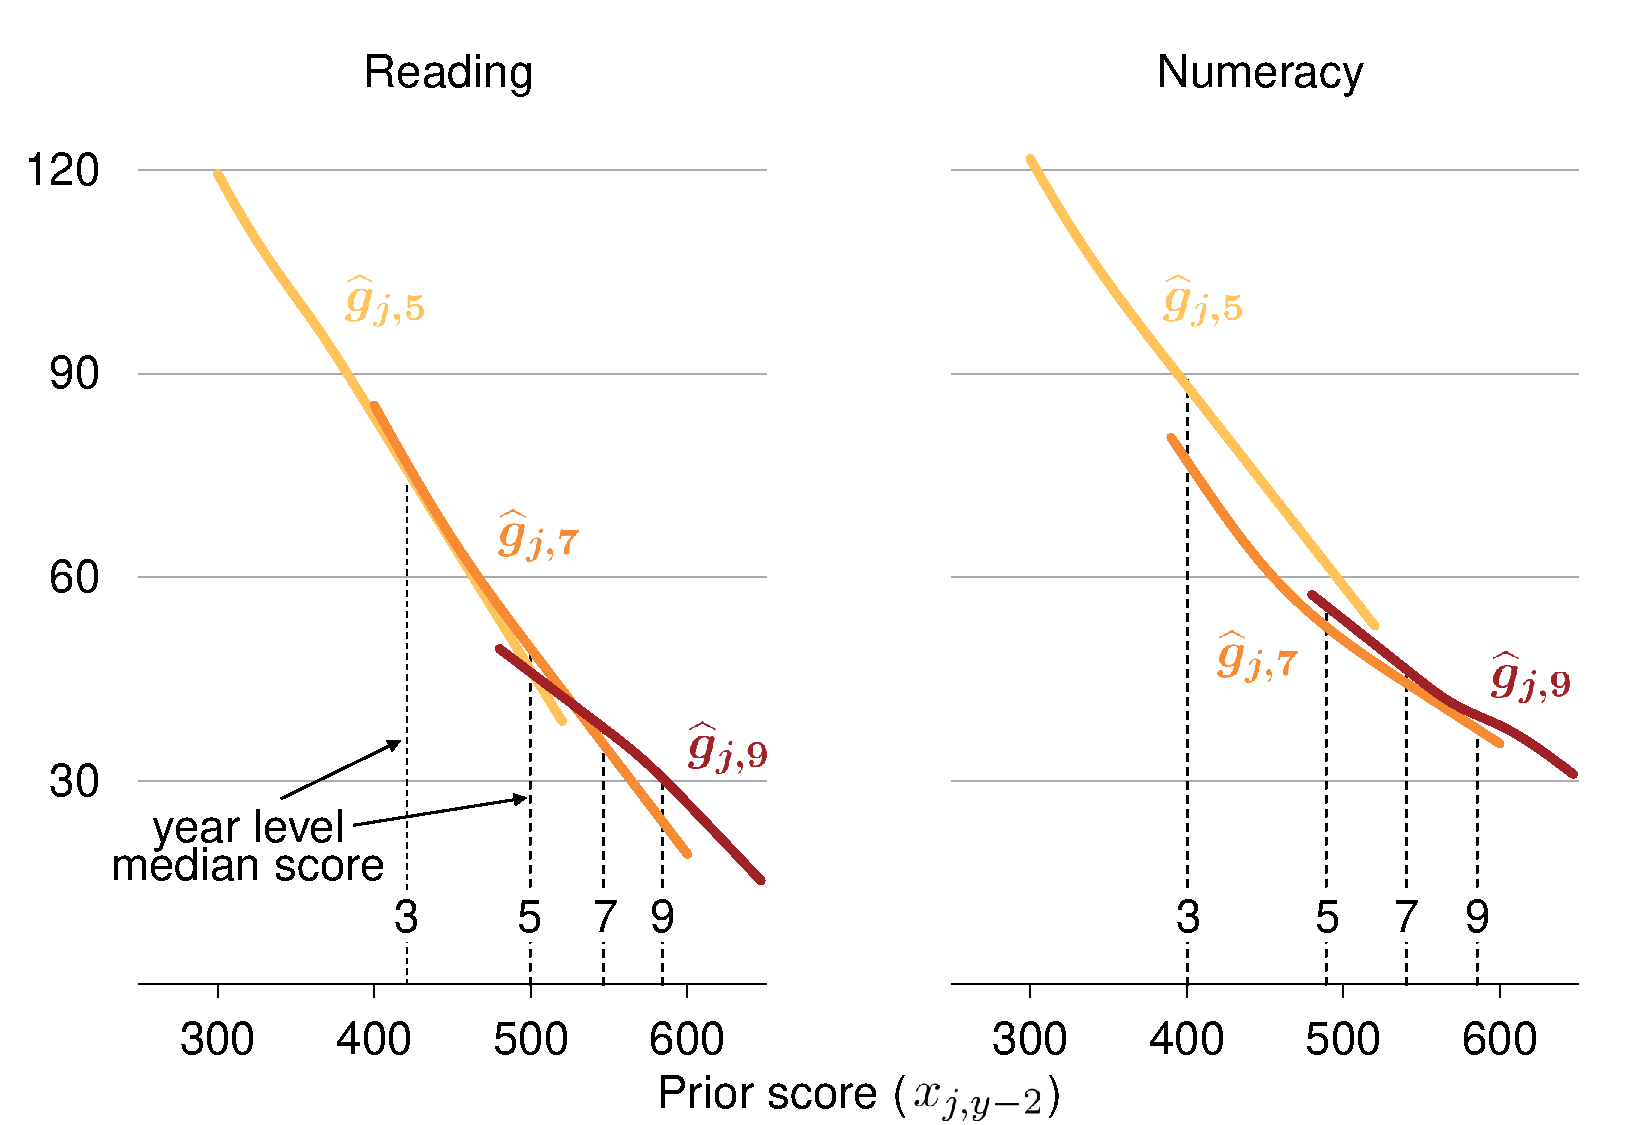
\includegraphics[width=\columnwidth]{atlas/G579.pdf}\label{fig:g579}

\source{Grattan analysis of \textcite{acara2014}.}
\end{figure}

Setting $Y=10$ and re-arranging \cref{eq:gf} gives:
\begin{equation}
f_{j}\left(10\right) = f_{j}\left(8\right) + g_{j,10}\left[f_{j}\left(8\right)\right]
\end{equation}
The point $f_{j}\left(8\right)$ was estimated in Step 2, but it is not possible to estimate $g_{j,10}$ without NAPLAN data for Year 10 students (linked to Year 8 results). But given that year level has little effect on gain scores once prior scores are controlled for, we can assume:
\begin{equation}
g_{j,10}\left[f_{j}\left(8\right)\right] \approx g_{j,9}\left[f_{j}\left(8\right)\right] \label{eq:g9g10}
\end{equation}
That is, our estimate of $g_{j,9}$ can be used as a proxy for $g_{j,10}$. In other words, we assume that a student in Year 8 performing at the median Year 8 level will make a similar gain over two years as a Year 7 student performing at the median Year 8 level.

Similarly, we can use our estimate of $g_{j,5}$ as a proxy for $g_{j,4}$ by assuming:
\begin{equation}
g_{j,4}\left[f_{j}\left(2\right)\right] \approx g_{j,5}\left[f_{j}\left(2\right)\right] \label{eq:g4g5}
\end{equation}
That is, a Year 2 student performing at the median Year 2 level is assumed to make a similar gain over two years as a Year 3 student performing at the median Year 2 level.

These approximations can be extended to further year levels outside the range of Year 3 to Year 9. For instance, $g_{j,9}$ can also be used to approximate $g_{j,11}$ and $g_{j,12}$.\footnote{The further away from the Year 3 to Year 9 range, the less accurate these approximations are likely to be. For instance, $\widehat{g}_{j,9}$ is probably not going to be a good proxy for $\widehat{g}_{j,13}$.}

\textbf{Step 4: Estimate the corresponding NAPLAN scale scores for comparative year levels 10, 11, and 12}
\nopagebreak

Using the assumption made in \cref{eq:g9g10} and its extensions, $f_{j}(10),f_{j}(11)$ and $f_{j}(12)$ are estimated using the following:
\begin{equation} \begin{array}{c}
\widehat{f}_{j}\left(10\right) = \widehat{f}_{j}\left(8\right) + \widehat{g}_{j,9}\left[\widehat{f}_{j}\left(8\right)\right] \vspace{0.3em}\\
\widehat{f}_{j}\left(11\right) = \widehat{f}_{j}\left(9\right) + \widehat{g}_{j,9}\left[\widehat{f}_{j}\left(9\right)\right] \vspace{0.3em}\\
\widehat{f}_{j}\left(12\right) = \widehat{f}_{j}\left(10\right) + \widehat{g}_{j,9}\left[\widehat{f}_{j}\left(10\right)\right]
\end{array} \end{equation}
where, for example, $\widehat{f}_{j}(8)$ is the estimated median NAPLAN scale score for Year 8 students, calculated in Step 2, and $\widehat{g}_{j,9}$ is the estimated median NAPLAN gain score from Year 7 to Year 9, calculated in Step 3. It is necessary to calculate $\widehat{f}_{j}(10)$ before calculating $\widehat{f}_{j}(12)$.

\textbf{Step 5: Estimate the corresponding NAPLAN scale scores for comparative year levels 1.5, 2, and 2.5}
\nopagebreak

Using the assumption made in \cref{eq:g4g5} and its extensions, $f_{j}(1.5),f_{j}(2)$ and $f_{j}(2.5)$ are estimated by solving the following equations for $\widehat{f}_{j}\left(Y\right)$:
\begin{equation} \begin{array}{c}
\widehat{f}_{j}\left(1.5\right) = \widehat{f}_{j}\left(3.5\right) - \widehat{g}_{j,5}\left[f_{j}\left(1.5\right)\right] \vspace{0.3em}\\
\widehat{f}_{j}\left(2\right) = \widehat{f}_{j}\left(4\right) - \widehat{g}_{j,5}\left[f_{j}\left(2\right)\right] \vspace{0.3em}\\
\widehat{f}_{j}\left(2.5\right) = \widehat{f}_{j}\left(4.5\right) - \widehat{g}_{j,5}\left[f_{j}\left(2.5\right)\right]
\end{array} \end{equation}
where, for example, $\widehat{f}_{j}(3.5)$ is the estimated median NAPLAN scale score for Year 3 students, six months after the NAPLAN test (November), and $\widehat{g}_{j,5}$ is the estimated median gain score from Year 3 to Year 5, calculated in Step 3. The points are estimated closer together because $f_{j}(Y)$ has a larger gradient for lower values of $Y$.

\textbf{Step 6: Interpolate over estimated points}
\nopagebreak

Using a range of estimated points for $\left[Y,\widehat{f}_{j}(Y)\right]$ (for example, use $Y$ = 1.5, 2, 2.5, 3, 4, 5, 6, 7, 8, 9, 10, 11, 12), construct a smooth curve for $\widehat{f}_{j}(Y)$ using interpolation.\footnote{Our methodology fits a curve using a regression with restricted cubic splines -- some of the points already estimated for $f_{j}(Y)$ shift slightly as a result.} We extrapolate our curve so that $y_{min} = 1$ and $y_{max} = 13$ (reported as `above Year 12'), although our analysis aims to avoid these extremes as much as possible given the high standard errors associated with these estimates.\footnote{Given that NAPLAN is designed for students between Year 3 and Year 9, not only are estimates less reliable outside this range, but the interpretation of comparative year levels becomes more difficult as we move further outside this range.}

We now have a curve that estimates the median NAPLAN scale score for each schooling year level: $\widehat{f}_{j}(Y)$. The inverse of this curve is used to estimate the comparative year level, $Y^{*}$, corresponding to any given NAPLAN scale score, $X_{j}$:
\begin{equation} \widehat{Y}^{*} = \widehat{f}_{j}^{-1}(X_{j}) \end{equation}

\begin{figure}[t]
 \captionwithunits{All NAPLAN scale scores correspond to a comparative year level}{Median NAPLAN scale score \hspace{2.4em} Comparative year level ($\widehat{Y}^{*}$}
% \vspace{-1.2em}
 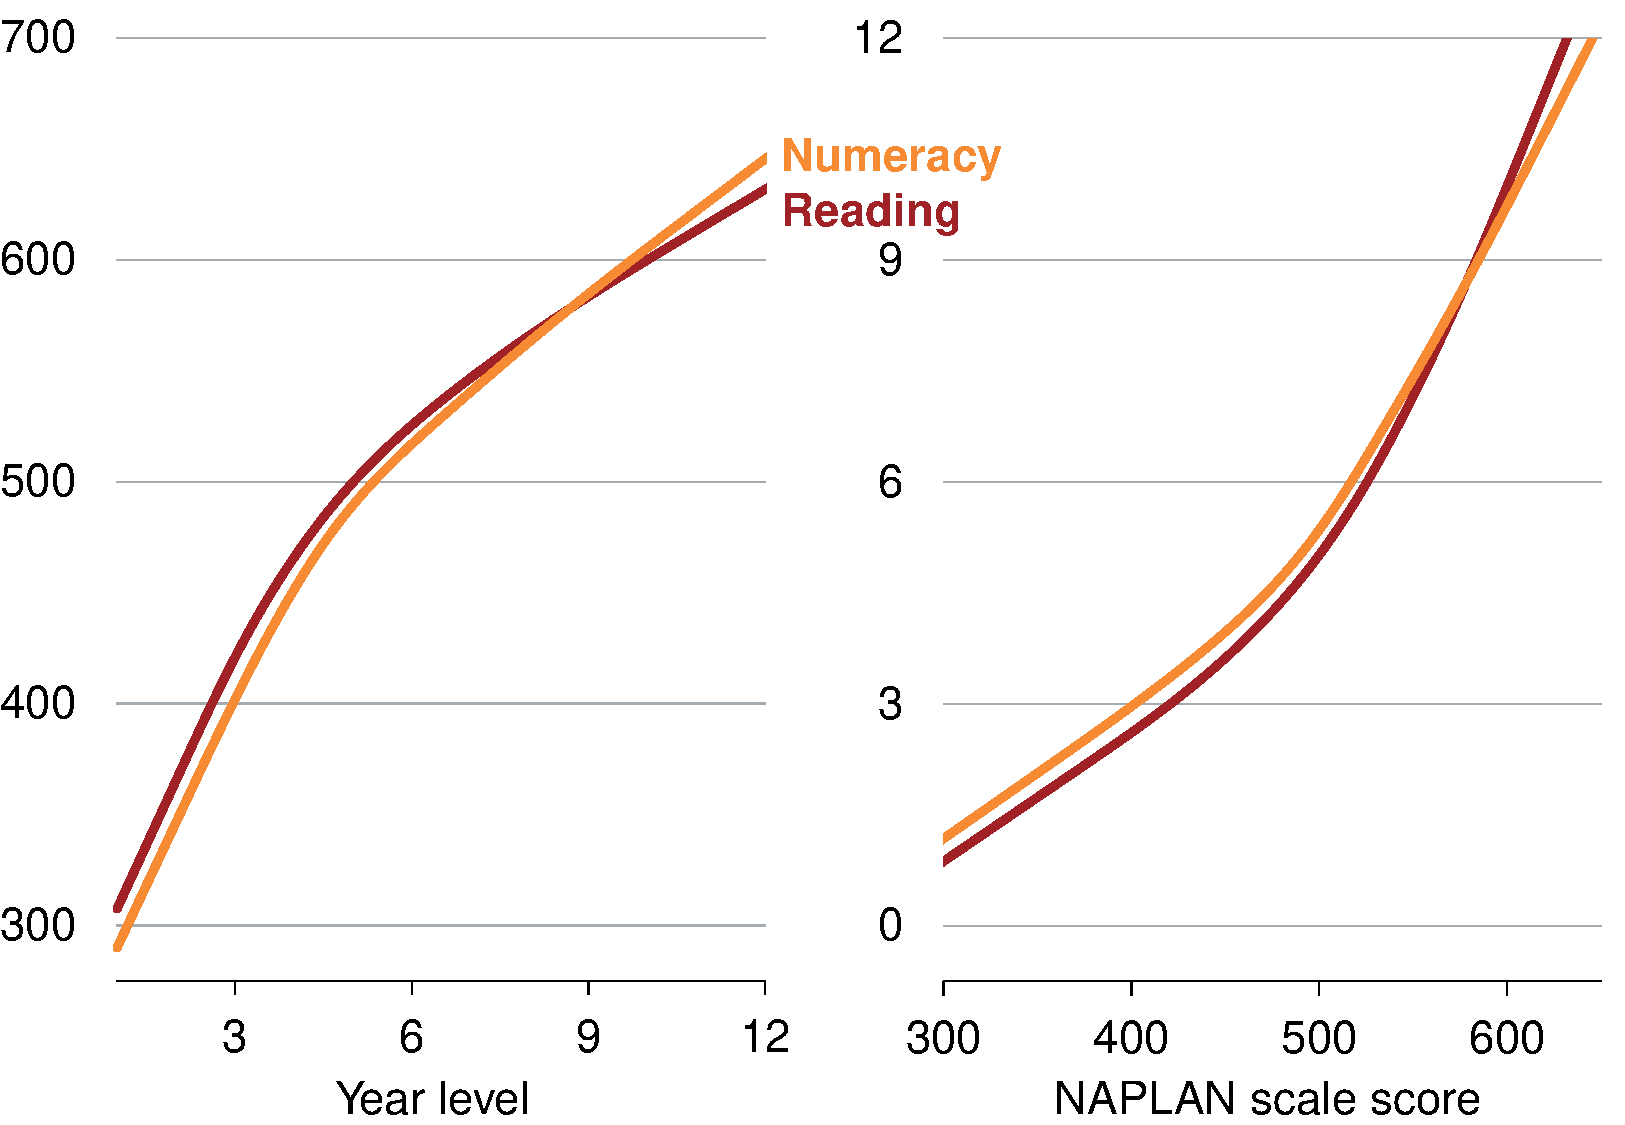
\includegraphics[width=\columnwidth]{atlas/CYL_and_inverse.pdf}\label{fig:cyl_inverse}
\notes{Left chart shows estimated function $\widehat{f}_{j}(Y)$, while right chart shows its inverse, $\widehat{f}_{j}^{-1}(X_{j})$. The left chart can be interpreted as the estimated median NAPLAN scale score for a given year level, whereas the right chart can be interpreted as the estimated comparative year level for a given NAPLAN scale score.}

\source{Grattan analysis of \textcite{acara2014}.}
\end{figure}

\Cref{fig:cyl_inverse} shows this curve for reading and numeracy, both in terms of $\widehat{f}_{j}(Y)$ and in terms of its inverse, $\widehat{f}_{j}^{-1}(X_{j})$. As the right chart shows, every NAPLAN score (within the range of the curve) can be mapped to a comparative year level. A score of 500 in numeracy, for instance, corresponds to a comparative year level of 5 years and 4 months -- a student at this level can be interpreted as performing four months ahead of the typical (median) Year 5 student at the time of the Year 5 NAPLAN test.\footnote{Given that NAPLAN is administered in May of each year, another interpretation is to say that this student is performing at the level we'd expect of the typical Year 5 student in September.}

These curves can be used to compare different cohorts or sub-groups of students in terms of differences in their achievement, and to track student progress relative to the median student. Years of progress is simply calculated as the difference in comparative year levels between two points in time. If, for example, a student makes 2 years and 6 months of progress over a two-year period, they have made the same amount of progress as we'd expect the typical (median) student to make over 2 years and 6 months, starting from the same point. This student could be said to be learning 25 per cent faster than the typical student.

\section{Robustness of comparative year level estimates}

There are a number of questions that may arise in relation to the methodology used to estimate comparative year levels. For instance:
\begin{itemize}
    \item what is the standard error around point estimates?
    \item how accurate are estimates beyond Year 3 and Year 9?
    \item how do the estimates change with different assumptions?
    \item are the results robust to the cohort used?
\end{itemize}

It is worth investigating each of these questions in detail to ensure that the methodology and the results are robust.

\subsection{Standard errors around point estimates}

There are two sources of error that the standard error accounts for: sample size and measurement error. But the comparative year level curve is calculated from a very large sample, meaning that standard errors due to both sources are naturally small.

In reporting, we prefer using confidence intervals to standard errors, since comparative year levels are asymmetrically distributed around NAPLAN scale scores. We calculate a 99 per cent confidence interval at each point along the curve, $\widehat{f}_{j}(Y)$, between $Y=1$ and $Y=13$. This is based on a bootstrap simulation with 200 replications.\footnote{Each replication uses a different set of random draws. The lower bound at each point is the average of the two lowest simulated points, while the upper bound at each point is the average of the two highest simulated points.}

Between Year 3 and Year 9, comparative year levels are estimated within a month of learning. As the curve is flatter in Year 9 than it is in Year 3, the confidence interval around Year 9 is wider. The width of the confidence interval naturally increases as you go below Year 3 or above Year 9. But the interval is widest when estimating comparative year level 1: three months for numeracy, and six months for reading, as shown in \Cref{fig:cyl_ci}. At comparative year level 13, the width of the confidence interval is two months for numeracy, and three months for reading, reflecting that there are still a significant number of students who reach this level by Year 9.

The confidence intervals for each comparative year level are displayed in \Cref{tab:cyl_ci}.

\begin{figure}[t]
 \captionwithunits{Confidence intervals are widest for low NAPLAN scale scores}{Comparative year level with 99 per cent confidence interval}
% \vspace{-1.2em}
 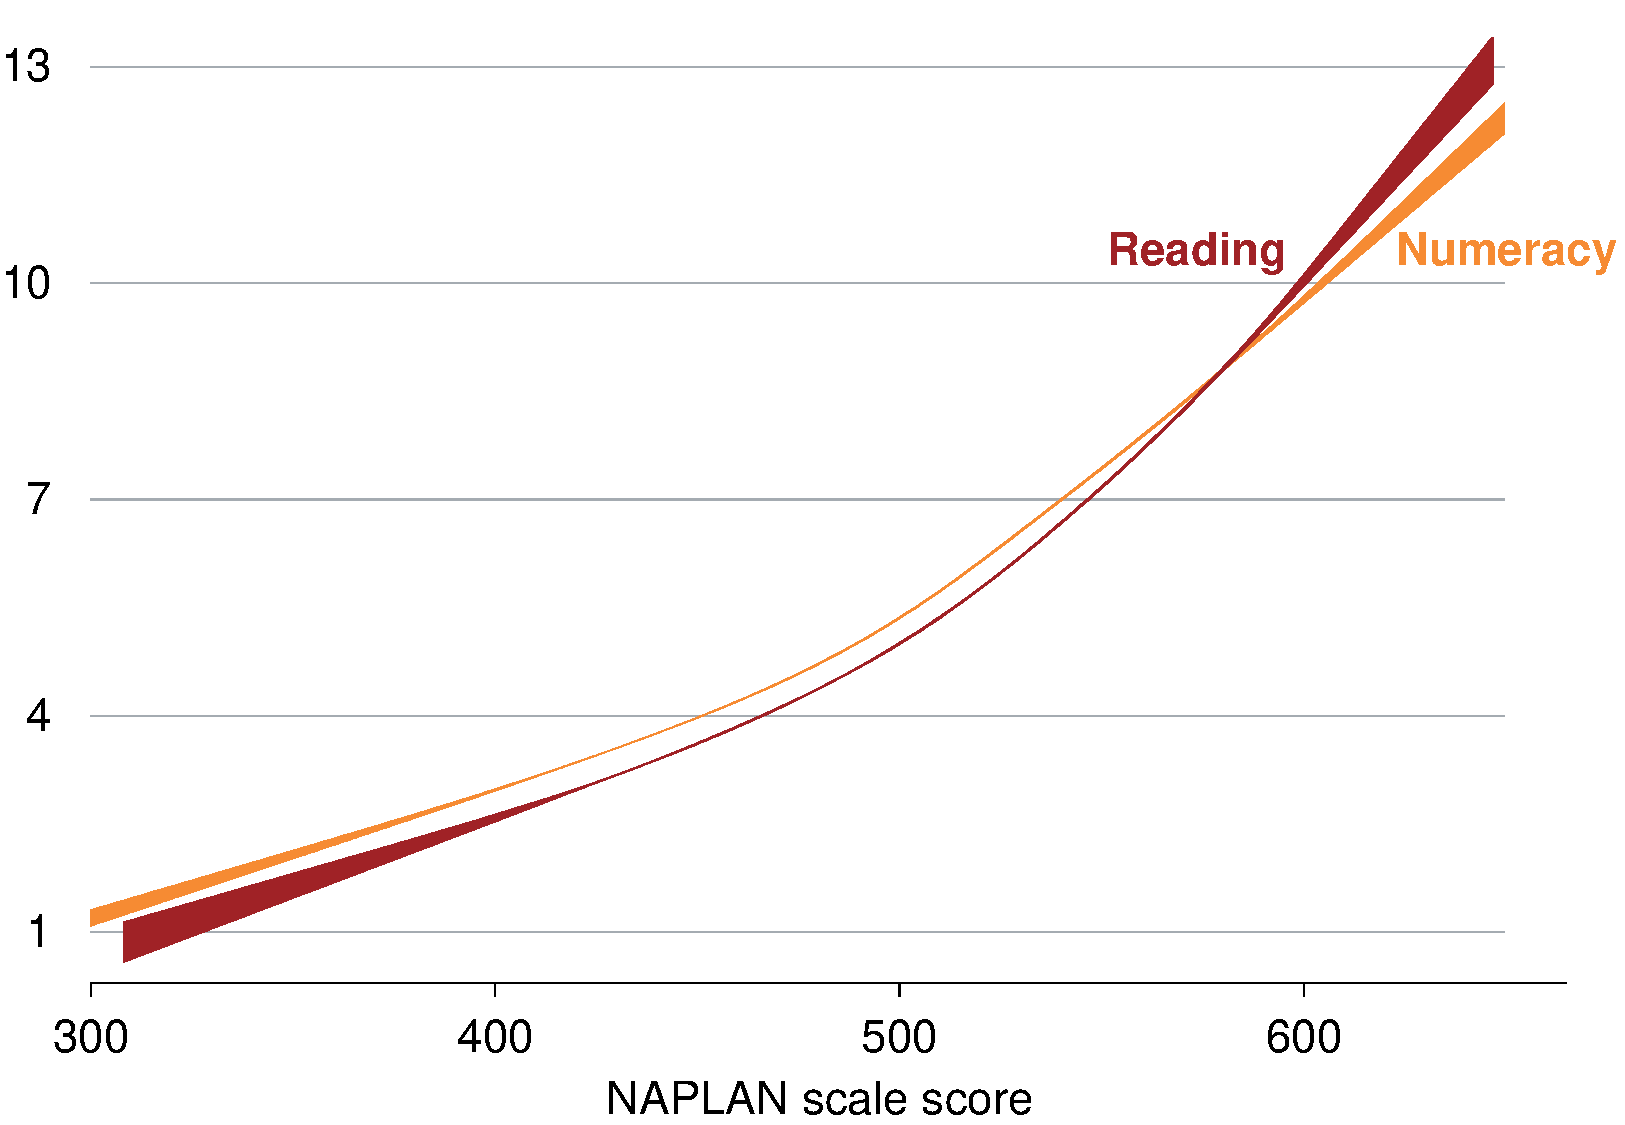
\includegraphics[width=\columnwidth]{atlas/CYL_CI.pdf}\label{fig:cyl_ci}
\notes{Confidence intervals become wider for comparative year levels greater than Year 9, but are not as wide as they are for low year levels.}

\source{Grattan analysis of \textcite{acara2014}.}
\end{figure}

\begin{table}[h]
  \centering
  \caption{Estimated comparative year levels with 99 per cent confidence interval}
    \begin{tabular}{lclcl}

    Comp. year & \multicolumn{2}{c}{Numeracy} & \multicolumn{2}{c}{Reading} \\
    \cmidrule(lr){2-3} \cmidrule(lr){4-5}
      level ($\widehat{Y}^{*}$) & $\widehat{f}_{j}(Y)$ & \multicolumn{1}{c}{Interval} & $\widehat{f}_{j}(Y)$ & \multicolumn{1}{c}{Interval} \\ \midrule
    1     & 288.5 & (0.86,1.1) & 314.8 & (0.74,1.21) \\
    2     & 345.4 & (1.93,2.05) & 368.7 & (1.88,2.1) \\
    3     & 401.4 & (2.98,3.01) & 421.1 & (2.98,3.01) \\
    4     & 451.4 & (3.99,4.01) & 466.0 & (3.98,4.01) \\
    5     & 489.4 & (4.99,5.02) & 499.9 & (4.99,5.02) \\
    6     & 516.2 & (5.98,6.02) & 524.6 & (5.98,6.02) \\
    7     & 540.0 & (6.98,7.02) & 546.2 & (6.98,7.02) \\
    8     & 563.9 & (7.97,8.02) & 566.7 & (7.98,8.03) \\
    9     & 586.0 & (8.96,9.02) & 584.6 & (8.97,9.06) \\
    10    & 605.6 & (9.94,10.03) & 599.4 & (9.97,10.08) \\
    11    & 623.8 & (10.93,11.04) & 612.4 & (10.95,11.09) \\
    12    & 641.4 & (11.92,12.05) & 624.8 & (11.92,12.11) \\
    13    & 659.0 & (12.9,13.06) & 637.1 & (12.88,13.13) \\
    \bottomrule
    \end{tabular}%
  \label{tab:cyl_ci}%
\begin{flushleft}\notes{Parentheses show upper and lower bounds of 99 per cent confidence interval for estimated comparative year levels. This is estimated by a bootstrap simulation with 200 replications.}

\source{Grattan analysis of \textcite{acara2014}.}\end{flushleft}
\vspace{-6pt}
\end{table}%

It should be noted that these confidence intervals are calculated assuming that the methodology is correct. If we were to account for uncertain assumptions, the intervals would be wider.\footnote{The narrow confidence intervals tell us that error due to measurement and sample size is very small. They do not tell us whether or not the methodology is appropriate.}

\subsection{Accuracy of estimates beyond Year 3 and Year 9}

Without students taking a NAPLAN test outside of the test-taking years, it is impossible to validate whether our estimates of the median NAPLAN scale score in Years 1, 2, 10, 11, and 12 reflect how the median student would actually perform in those year levels. But it is possible to use a similar methodology to predict the median score in Year 3 and Year 9 without using data from Year 3 and Year 9.

Using data for students in Year 7 linked to their Year 5 results, \Cref{fig:57} shows that the methodology does a reasonable job of estimating the curve outside the years that data are available. Interestingly, the curve estimated with only Years 5 and 7 overestimates the median score at both the bottom and the top of the curve.\footnote{This is the opposite of what is expected due to regression to the mean.} 

\begin{figure}[t]
 \captionwithunits{Data from Years 5 and 7 students will slightly overestimate the median score for year levels outside the range}{Estimated median NAPLAN scale score, reading}
% \vspace{-1.2em}
 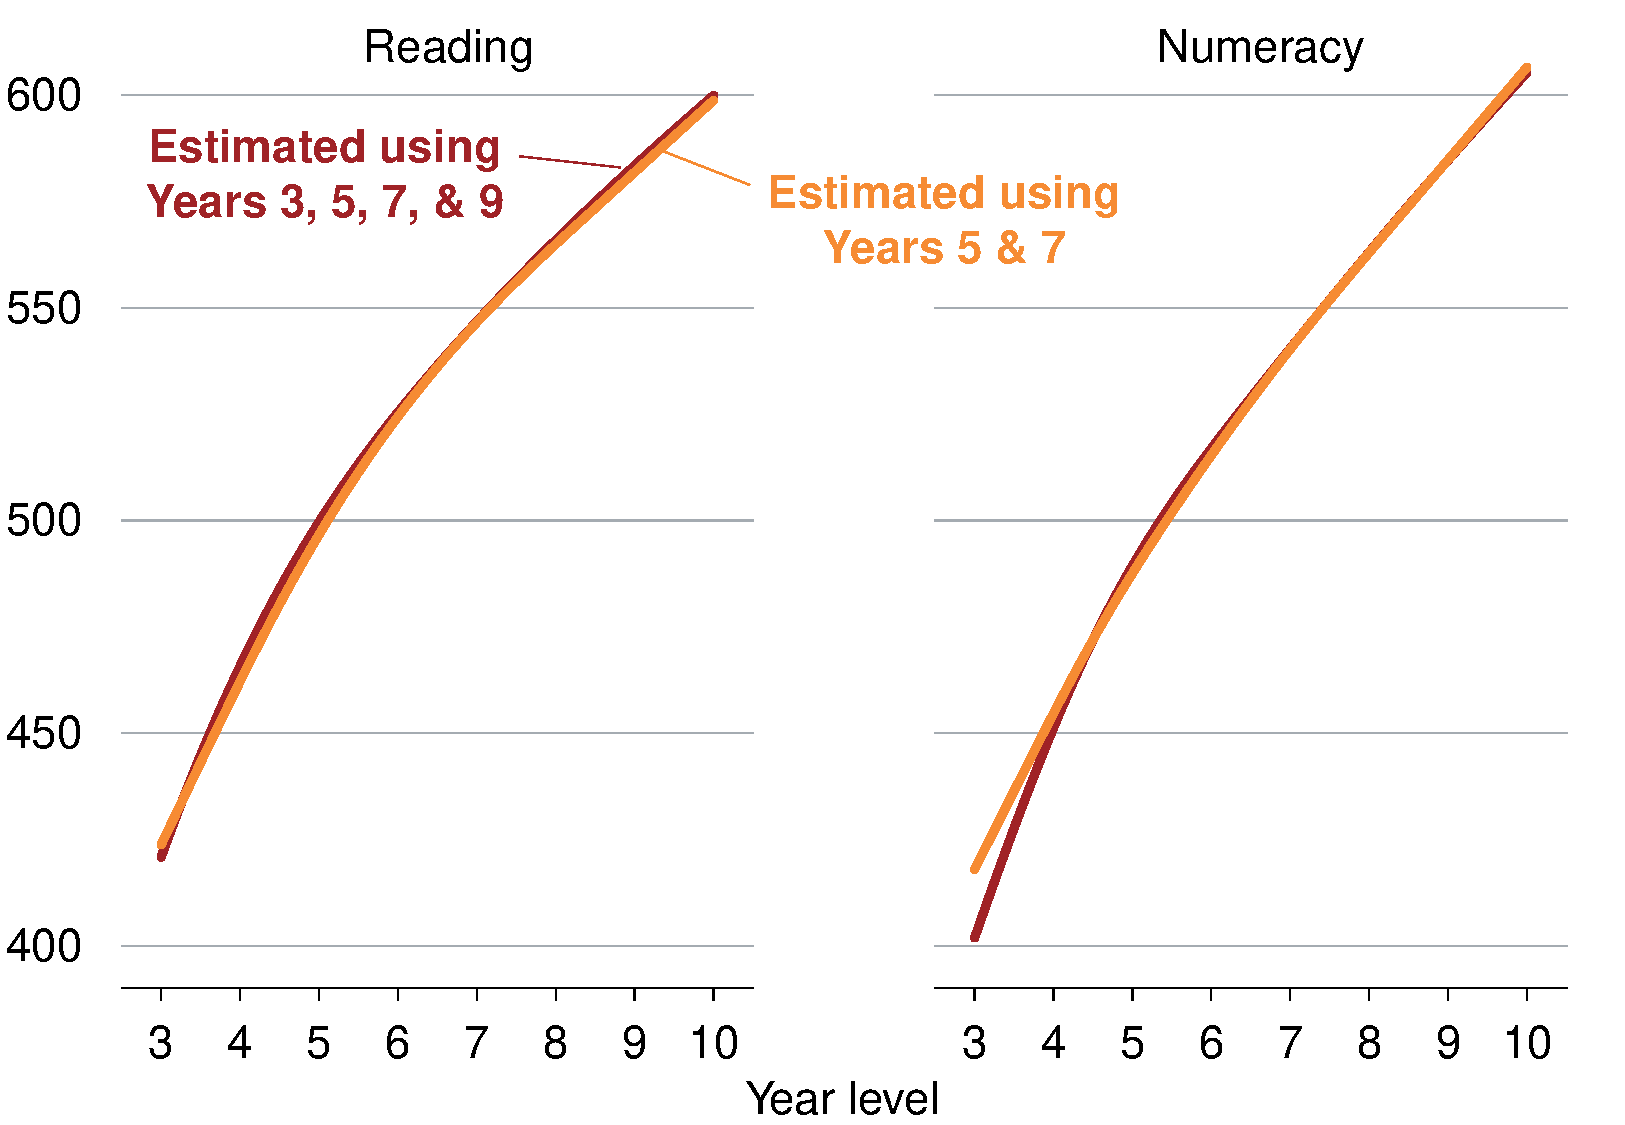
\includegraphics[width=\columnwidth]{atlas/five_seven.pdf}\label{fig:57}
\notes{Overestimating the median score at high and low year levels will lead to conservative estimates of the gap between high and low achievers in terms of years of progress. A similar pattern holds for numeracy.}

\source{Grattan analysis of \textcite{acara2014}.}
\end{figure}

\subsection{How do estimates change with different assumptions?}

\verb+to be completed+

\subsection{How robust are estimates to different cohorts}

\verb+2013 data linked to 2011 -- numeracy curve is flatter at the top+

\section{How comparative year levels could be implemented as part of NAPLAN reporting}

\begin{itemize}
    \item inital curve could be based on multiple cohorts (to improve robustness, since there are cohort specific effects)
    \item having calculated an initial curve, this should be fixed over time to track system-level improvements
    \item curves could be calculated using plausible values
    \item for individuals or schools, could track progress relative to a different percentile 
\end{itemize}












